
\documentclass{jtetiproposalskripsi}

%-----------------------------------------------------------------
%Disini awal masukan untuk data proposal skripsi
%-----------------------------------------------------------------
\titleind{SISTEM INFORMASI PERPUSTAKAAN BERBASIS WEB PADA SMPN 1 BANGSALSARI}
\fullname{ADE MUCHTAR}

\idnum{1200631008}

\approvaldate{14 Januari 2015}

\degree{Sarjana Teknik Elektro}

\yearsubmit{2015}

\program{Manajemen Informatika}

\headprogram{Triawan Adi Cahyadi,M.Kom}

\dept{Manajemen Informatika }

\firstsupervisor{Triawan Adi Cahyadi,M.Kom.}
\firstnip{12 03 719}

\secondsupervisor{Bagus Setya Rintyarna,ST,M.Kom}
\secondnip{09 03 521}


%-----------------------------------------------------------------
%Disini akhir masukan untuk data proposal skripsi
%-----------------------------------------------------------------

\begin{document}

\cover

\approvalpage

%-----------------------------------------------------------------
%Disini akhir masukan untuk muka skripsi
%-----------------------------------------------------------------

%-----------------------------------------------------------------
%Disini awal masukan Intisari
%-----------------------------------------------------------------
\begin{abstractind}
Perpustakaan biasanya difungsikan oleh pengunjung sebagai media mencari referenci dan memperoleh informasi.Permasalahan yang dihadapi saat ini adalah banyaknya perpustakaan di sekolah-sekolah yang belum memiliki sistem informasi perpustakaan yang berbasis web.Di smp negeri 1 bangsalsari merupakan salah satu sekolah yang belum menggunakan sistem informasi perpustakaan berbasis web sebagai media untuk memberi informasi kepada siswa-siswinya.

Dengan menggunakan perangkat lunak  Macromedia Dreamweaver, PHP dan MySQL  sebagai media untuk mengembangkan sistem informasi perpustakaan berbasis web penulis bertujuan untuk mengembangkan perpustakan di smp negeri 1 bangsalsari ke sistem informasi perpustakaan yang berbasis web.

Objektif utama sistem informasi ini adalah agar kinerja pengolahan data bahan pustaka,pencarian buku dan peminjaman buku dapat ditingkatkan dan siswa-siswa lebih mudah dan tidak membosankan untuk membaca ataupun mencari buku melalui sistem informasi.


\bigskip
\textbf{Kata kunci} : perpustakaan,smp negeri 1 bangsalsari,macromedia ,php,dan mysql.
\end{abstractind}
%-----------------------------------------------------------------
%Disini akhir masukan Intisari
%-----------------------------------------------------------------

\tableofcontents
\addcontentsline{toc}{chapter}{DAFTAR ISI}
\selectlanguage{bahasa}\clearpage\pagenumbering{arabic}\setcounter{page}{1}

%-----------------------------------------------------------------
%Disini awal masukan untuk Bab
%-----------------------------------------------------------------
\chapter{LATAR BELAKANG}

\section{Latar Belakang Masalah}
Keberadaan perpustakaan sekolah di Indonesia saat ini masih berada dalam tahap perkembangan. Oleh karena itu sebagai komponen pendidikan yang turut mendukung kegiatan proses belajar mengajar memerlukan banyak perhatian dan dukungan dari berbagai pihak.

Pasal 35 UU No. 2 Tahun 1989 tentang Sistem Pendidikan Nasional menetapkan bahwa: Setiap satuan pendidikan sekolah, baik yang diselenggarakan oleh pemerintah maupun masyarakat harus menyediakan sumber belajar. Oleh karena itu Pendidikan tidak mungkin terselenggara dengan baik apabila para tenaga kependidikan maupun peserta didik tidak didukung oleh sumber belajar yang diperlukan untuk penyelenggaraan kegiatan belajar mengajar yang bersangkutan.

Undang-undang RI Nomor 43 Tahun 2007 tentang Perpustakaan pasal 23 ayat (1) menyebutkan definisi perpustakaan sekolah sebagai berikut: Setiap sekolah/madrasah menyelenggarakan perpustakaan yang memenuhi standar nasional perpustakaan dengan memperhatikan standar nasional pendidikan.

Dalam era globalisasi sekarang ini dunia informasi berkembang begitu pesat karena ditunjang dengan perkembangan teknologi yang semakin canggih. Komputer merupakan salah satu alat yang digunakan untuk menunjang perkembangan teknologi informasi. Oleh karena itu suatu lembaga yang menggunakan komputer dalam mengelola sistem informasinya akan mempunyai nilai lebih daripada sistem yang diolah secara manual. Dapat dikatakan sistem informasi yang menggunakan komputer akan menunjang efisiensi dan produktivitas yang tinggi.

Kegiatan administrasi yang dilakukan oleh perpustakaan sekolah merupakan kegiatan pelayanan utama di SMPN 1 BANGSALSARI. Salah satu pelayanan yang diberikan pihak sekolah kepada para murid adalah menyediakan  referensi akademik dalam bentuk penyediaan buku-buku di perpustakaan. Para siswa diberi kesempatan untuk memanfaatkan berbagai macam buku yang disediakan di perpustakaan dengan sistem peminjaman periodik.
Sesuai dengan uraian di atas, penulis merasa perlu untuk membahas lebih mendalam mengenai sistem Perpustakaan di SMPN 1 Bangsalsari dalam pembuatan tugas akhir dengan mengambil judul \textbf{SISTEM INFORMASI PERPUSTAKAAN BERBASIS WEB PADA SMPN 1 BANGSALSARI}.

\section{Rumusan Masalah}
Dari uraian Latar Belakang Masalah di atas, penulis dapat mengidentifikasikan masalah sebagai berikut:
\begin{itemize}
\item[1.]Belum terintegrasinya data-data buku pada perpustakaan sekolah, sehingga keberadaannya tidak teratur.
\item[2.]Tidak terdapat penyimpanan data berbasis database, sehingga proses pengolahan dan pencarian data menjadi lama.
\item[3.]Lambatnya proses pengolahan, sehingga data dan informasi yang dihasilkan kurang akurat dan aktual.

\end{itemize}

\section{Batasan Masalah}
Supaya pembahasan masalah yang dilakukan dapat terarah dengan baik dan tidak menyimpang dari pokok permasalahan, maka penulis membatasi permasalahan yang akan dibahas, yakni:
\begin{itemize}
\item[1.]Aplikasi ini dibangun dengan menggunakan PHP sebagai Server Side Programming Language dan MySQL sebagai database servernya.
\item[2.]Sistem yang dibuat terdiri dari Data User, Data Buku, Data Anggota / Peminjam, Data Peminjaman Buku dan Data Pengembalian Buku.
\item[3.]Pencetakan Laporan meliputi Laporan Data Buku, Laporan Data Anggota / Peminjam, Laporan Data Peminjaman Buku, Laporan Data Pengembalian Buku dan Laporan Pendapatan / Denda.
\end{itemize}


\section{Tujuan Penelitian}
Tujuan yang hendak dicapai dalam perancangan Sistem Informasi Perpustakaan ini adalah sebagai berikut:
\begin{itemize}
\item[1.]Untuk mengetahui sistem administrasi perpustakaan yang diterapkan pada smpn 1 bangsalsari.
\item[2.]Sebagai sarana untuk memudahkan penginputan dan pengolahan data, agar meminimalisir terjadinya kesalahan.
\item[3.]Agar dihasilkan laporan-laporan yang lebih cepat dan akurat.
\end{itemize}


\section{Manfaat Penelitian}
\begin{itemize}
\item[1.]Membantu petugas perpustakaan dalam melakukan pengolahan data di
perpustakaan SMPN 1 Bangsalsari .
\item[2.]Memberikan kemudahan pengunjung untuk mendapatkan informasi-informasi
bahan pustaka dan memberikan kemudahan dalam melakukan pendaftaran
dan melakukan transaksi peminjaman atau pengembalian bahan pustaka
\end{itemize}


\section{Metodelogi Penelitian}
Metoda pengumpulan data yang dilakukan dalam penelitian ini adalah:
\begin{itemize}
\item[1.]Observasi
Pengumpulan data dengan dengan melakukan pengamatan secara langsung terhadap objek penelitian, dengan mencatat hal-hal penting yang berhubungan dengan judul laporan, sehingga diperoleh data yang lengkap dan akurat.

\item[2.]Wawancara
Pengumpulan data dengan cara melakukan komunikasi dan wawancara secara langsung dengan pihak-pihak terkait.

\item[3.]Studi Pustaka

Pengumpulan data dengan menggunakan atau mengumpulkan sumber-sumber tertulis, dengan cara membaca, mempelajari dan mencatat hal-hal penting yang berhubungan dengan masalah yang sedang dibahas guna memperoleh gambaran secara teoritis.
\end{itemize}


%-------------------------------------------------------------------------------
\chapter{Landasan Teori}          
\section{Konsep Dasar Sistem}      
Pengertian sistem pada berbagai bidang berbeda-beda, tetapi meskipun
istilah sistem yang digunakan bervariasi, semua sistem pada bidang-bidang tersebut mempunyai beberapa persyaratan umum, yaitu sistem harus mempunyai elemen, lingkungan, interaksi antar elemen, interaksi antara elemen dengan lingkungannya, dan yang terpenting adalah sistem harus mempunyai tujuan yang akan dicapai. Berdasarkan persyaratan ini, sistem dapat didefinisikan sebagai sekumpulan elemen-elemen (subsistem) yang berinteraksi dengan maksud yang sama untuk mencapai suatu tujuan tertentu. Kumpulan elemen terdiri dari manusia, mesin, prosedur, dokumen, data atau elemen lain yang terorganisir dari elemen-elemen tersebut. Elemen sistem disamping berhubungan satu sama lain, juga berhubungan dengan lingkungannya untuk mencapai tujuan yang telah ditentukan sebelumnya. 

\section{Konsep Dasar Informasi}
Informasi adalah sekumpulan data yang diproses sebagai tambahan pengetahuan untuk membantu pengambilan keputusan. Kualitas Informasiterdiri dari :
\begin{itemize}
\item[a)]Akurat 
\item[b)]Tepat pada waktunya 
\item[c)]Relevan 
\end{itemize}

\section{Konsep Dasar Sistem Informasi}
Sistem informasi dapat didefinisikan sebagai kumpulan komponen yang digunakan untuk mengolah data sehingga menghasilkan suatu informasi yang dapat digunakan untuk pengambilan keputusan. Komponen sistem informasi terdiri dari : 
\begin{itemize}
\item[1.] Orang-orang (brainware) 
Yang terlibat dalam pembuatan/penggunaan sistem informasi adalah sbb: 
\begin{itemize}
\item{} Data Processing Manager 
\item{} System Analyst 
\item{} Programmers 
\item{} Machine Operator 
\item{} Data Entry Operator 
\item{} System Administrator
\end{itemize}


\item[2.] Hardware 
Hardware dalam komponen sistem informasi dapat di golongkan menjadi beberapa bagian, yaitu: Media input, storage, proses dan media output 
\item[3.] Aturan 
Merupakan aturan-aturan yang digunakan sebagai pedoman dalam pengembangan sistem informasi. 
\item[4.] Software 
Software merupakan kumpulan dari perintah /fungsi yang ditulis dengan aturan tertentu untuk memerintahkan komputer melaksanakan tugas tertentu. Software terdiri dari : 
\begin{itemize}
\item[a.]	Sistem Software 
\begin{itemize}
\item{}	Operating Sistem 
\item{}	Tool/Utility 
\item{}	Programming Language 
\end{itemize}
\item[b.]	Application software 
\begin{itemize}
\item{}	Aplikasi umum 
\item{}	Aplikasi khusus 
\end{itemize}
\end{itemize}

\item[5.] Data 
Merupakan komponen dari informasi yang akan diproses lebih lanjut untuk menghasilkan informasi. Data merupakan jembatan penghubung antara manusia dan mesin agar terjadi suatu proses pengolahan data. 
\end{itemize}

\section{Konsep Permodelan Sistem}
\subsection{Flowchart Sistem}
Flowchart Sistem merupakan bagan yang menunjukkan alur kerja atau apa yang sedang dikerjakan di dalam sistem secara keseluruhan dan menjelaskan urutan dari prosedur-prosedur yang ada di dalam sistem. 
\subsection{Data Flow Diagram}
DFD merupakan alat perancangan sistem yang berorientasi pada alur data dengan konsep dekomposisi dapat digunakan untuk penggambaran analisa maupun rancangan sistem yg mudah dikomunikasikan oleh professional sistem kepada pemakai maupun pembuat program. 

\section{Konsep Basis Data}
\subsection{Definisi Basis Data}
Basis data adalah suatu susunan/kumpulan data operasional lengkap dari suatu organisasi/perusahaan yang diorganisir/dikelola dan disimpan secara terintegrasi dengan menggunakan metode tertentu menggunakan computer sehingga mampu menyediakan informasi optimal yang diperlukan pemakainya.
Sistem Basis Data adalah suatu sistem menyusun dan mengelola record-record menggunakan computer untuk menyimpan atau merekam serata memelihara data operasional lengkap sebuah organisasi/perusahaan sehingga mampu menyediakan informasi yang optimal yang diperlukan pemakai untuk proses pengambilan keputusan.
\\

Terdapat 4 komponen pokok sistem basis data, yaitu :
\begin{itemize}
\item[a.] Data 
\item[b.] Hardware(perangkat keras) 
\item[c.] Software(perangkat lunak) 
\item[d.] User atau pemakai
\end{itemize} 
 
Pemakai basis data dibagi atas 3 klasifikasi, yaitu : 
\begin{itemize}
\item[a.] Database Administrator(DBA), orang atau tim yang bertugas mengelola sistem basis data secara keseluruhan. 
\item[b.] Programmer, orang atau tim yang bertugas membuat program aplikasi. 
\item[c.] End user, orang yang mengakses basis data melalui terminal dengan menggunakan query language atau program aplikasi yang dibuat programmer. 
\end{itemize}

\subsection{\textit{Entity Relationship Diagram (ERD)} }
\textit{Entity Relationship Diagram} merupakan diagram atau gambar yang mendeskripsikan hubungan antar penyimpanan. Entity Relationship Diagram digunakan untuk menunjukkan aturan-aturan yang ada pada sistem informasi yang akan dibangun serta hubungan antar data. 

\subsection{\textit{Structured Query Language (SQL)} }
\textit{Structured Query Language} merupakan subbahasa pemrograman yang khusus dipergunakan untuk memanipulasi basis data. SQL memiliki 3 kategori perintah :
\begin{itemize}
\item[a)]Data Definition Language (DDL), yakni perintah-perintah yang digunakan untuk mendefinisikan (menciptakan, tambah/mengubah/hapus) sturktur data/tabel 
item[b)]	Data manipulation language (DML), yakni perintah yang digunakan untuk memanipulasi database (melihat, menenusuri, filtering, summarize, perhitungan, dll) 
\item[c)]	Data Control Language (DCL), digunakan untuk mengedalikan database Bahasa yang mendukung SQL antara lain : V Basic, C++ Builder,Delphi, MySQL,ORACLE,PostGreeSQL,JAVA,dll 
\end{itemize} 

\section{Konsep Sistem Informasi Perpustakaan }
Sistem informasi perpustakaan merupakan perangkat lunak yang didesain khusus utntuk mempermudah pendataan koleksi perpustakaan, katalog data anggota, transaksi dan sirkulasi koleksi perpustakaan. Selain itu sistem informasi perpustakaan merupakan sistem yang terintegrasi untuk menyediakan informasi guna mendukung operasi, manajemen dan fungsi pengambilan keputusan dalam perpustakaan
\section{Pemrograman Web }
\subsection{HTML \textit{(Hypertext Markup Language)}}
HTTP \textit{(Hypertext Transfer Protokol)} merupakan protokol yang digunakan untuk mentransfer data antara web server ke web browser. Protokol ini mentransfer dokumen-dokumen Web yang berformat HTML. Hypertext MarkupLanguage atau HTML adalah bahasa yang digunakan untuk menulis dokumen- dokumen dalam bentuk hypertext. Dokumen-dokumen tersebut didistribusikan dengan World Wide Web dan dapat dilihat oleh klien-klien pada komputer. Dokumen HTML disebut Markup Language, karena HTML berfungsi untuk memperindah file teks biasa untuk ditampilkan pada program Web browser. 
\subsection{PHP Programming }
PHP merupakan singkatan dari \textit{Hipertext Preprocessor} yang berjalan disisi server \textit{(server side scripting)}. Kelebihan PHP diantaranya, dapat berjalan pada semua jenis sistem operasi, dapat mengolah data dengan tipe apapun, membuat halaman web lebih dinamis, menerima dan menciptakan cookies, dan lain lain. Selain itu, skrip PHP tidak akan terlihat disisi browser, karena dokumen yang berformat php dikembalikan web sever dalam format HTML. 
Script PHP ini mulai bekerja saat adanya request PHP file tersebut dari \textit{Web browser}. Web server kemudian akan memanggil file tersebut, dan akan membaca semua request dari atas sampai bawah. Mengeksekusi beberapa script command, dan mengirimkan hasilnya dalam sebuah halaman HTML melalui browser. 
\subsection{Web Server \textit{(Apache)} }
Web server adalah server yang melayani permintaan klien terdapat pada halaman web\textit{(web browser)} dan berkomunikasi dengan middleware untuk menterjemahkan kode-kode tertentu, menjalankan kode-kode tersebut dan memungkinkan berinteraksi dengan basis data, PHP atau ASP, jika ada permintaan dari browser, maka web server akan memproses permintaan itu kemudian memberikan hasil prosesnya berupa data yang diinginkan kembali ke browser. Data ini mempunyai format yang standar, disebut dengan format SGML \textit{(standar general markup language)}. Data yang berupa format ini kemudian akan ditampilkan oleh browser sesuai dengan kemampuan browser tersebut. Untuk berkomunikasi dengan client-nya (web browser) mempunyai protokol sendiri, yaitu HTTP \textit{(hypertext tarnsfer protocol)}. Dengan protokol ini, komunikasi antar web server dengan client-nya dapat saling dimengerti dan lebih mudah.Dalam sistem ini, web server yang banyak digunakan untuk PHP adalah Apache. Tugas utama apache adalah menghasilkan halaman web yang benar kepada client peminta, berdasarkan kode PHP yang dituliskan oleh pembuat web.
\subsection{Web Browser }
Web browser adalah perangkat lunak (software) disisi klien yang digunakan untuk mengakses informasi web, memformat teks dan menempatkan grafik pada layer. Ada beberapa jenis web browser yang dipakai sebagai sumber tampilan antara lain : \textit{Internet Explorer, Netscape Navigator, Mozila, Opera,} dsb.

\section{Sistem Perangkat Lunak }
\subsection{MySQL}
MySQL adalah sebuah implementasi dari sistem manajemen basisdata relasional (RDBMS) yang didistribusikan secara gratis dibawah lisensi GPL (General Public License). Setiap pengguna dapat secara bebas menggunakan MySQL, namun dengan batasan perangkat lunak tersebut tidak boleh dijadikan produk turunan yang bersifat komersial. MySQL sebenarnya merupakan turunan salah satu konsep utama dalam basisdata yang telah ada sebelumnya; SQL (Structured Query Language). SQL adalah sebuah konsep pengoperasian basisdata, terutama untuk pemilihan atau seleksi dan pemasukan data, yang memungkinkan pengoperasian data dikerjakan dengan mudah secara otomatis. Kehandalan suatu sistem basisdata (DBMS) dapat diketahui dari cara kerja pengoptimasi-nya dalam melakukan proses perintah-perintah SQL yang dibuat oleh pengguna maupun program-program aplikasi yang memanfaatkannya. Sebagai peladen basis data, MySQL mendukung operasi basisdata transaksional maupun operasi basisdata non-transaksional. Pada modus operasi non-transaksional, MySQL dapat dikatakan unggul dalam hal unjuk kerja dibandingkan perangkat lunak peladen basisdata kompetitor lainnya. Namun demikian pada modus non-transaksional tidak ada jaminan atas reliabilitas terhadap data yang tersimpan, karenanya modus nontransaksional hanya cocok untuk jenis aplikasi yang tidak membutuhkan reliabilitas data seperti aplikasi blogging berbasis web (wordpress), CMS, dan sejenisnya. Untuk kebutuhan sistem yang ditujukan untuk bisnis sangat disarankan untuk menggunakan modus basisdata transaksional, hanya saja sebagai konsekuensinya unjuk kerja MySQL pada modus transaksional tidak secepat unjuk kerja pada modus nontransaksional.
\\
MySQL memiliki beberapa keistimewaan, antara lain :
\begin{itemize}
\item[1.] \textbf{Portabilitas.} MySQL dapat berjalan stabil pada berbagai sistem operasi seperti Windows, Linux, FreeBSD, Mac Os X Server, Solaris, Amiga, dan masih banyak lagi.
\item[2.] \textbf{Perangkat lunak sumber terbuka.} MySQL didistribusikan sebagai perangkat lunak sumber terbuka, dibawah lisensi GPL sehingga dapat digunakan secara gratis.
\item[3.]\textbf{ Multi-user.} MySQL dapat digunakan oleh beberapa pengguna dalam waktu yang bersamaan tanpa mengalami masalah atau konflik.
\item[4.]\textbf{ 'Performance tuning',} MySQL memiliki kecepatan yang menakjubkan dalam menangani query sederhana, dengan kata lain dapat memproses lebih banyak SQL per satuan waktu.
\item[5.]\textbf{ Ragam tipe data.} MySQL memiliki ragam tipe data yang sangat kaya, seperti signed / unsigned integer, float, double, char, text, date, timestamp, dan lainlain.
\item[6.]\textbf{ Perintah dan Fungsi.} MySQL memiliki operator dan fungsi secara penuh yang mendukung perintah Select dan Where dalam perintah (query).
\item[7.]\textbf{ Keamanan.} MySQL memiliki beberapa lapisan keamanan seperti level subnetmask, nama host, dan izin akses user dengan sistem perizinan yang mendetail serta sandi terenkripsi.
\item[8.]\textbf{ Skalabilitas dan Pembatasan.} MySQL mampu menangani basis data dalam skala besar, dengan jumlah rekaman (records) lebih dari 50 juta dan 60 ribu tabel serta 5 milyar baris. Selain itu batas indeks yang dapat ditampung mencapai 32 indeks pada tiap tabelnya.
\item[9.]\textbf{ Konektivitas.} MySQL dapat melakukan koneksi dengan klien menggunakan protokol TCP/IP, Unix soket (UNIX), atau Named Pipes (NT).
\item[10.]\textbf{ Lokalisasi.} MySQL dapat mendeteksi pesan kesalahan pada klien dengan menggunakan lebih dari dua puluh bahasa. Meski pun demikian, bahasa Indonesia belum termasuk di dalamnya.
\item[11.]\textbf{ Antar Muka.} MySQL memiliki antar muka (interface) terhadap berbagai aplikasi dan bahasa pemrograman dengan menggunakan fungsi API (Application Programming Interface). 
\item[12.]\textbf{ Klien dan Peralatan.} MySQL dilengkapi dengan berbagai peralatan yang dapat digunakan untuk administrasi basis data, dan pada setiap peralatan yang ada disertakan petunjuk online.
\item[13.]\textbf{ Struktur tabel.} MySQL memiliki struktur tabel yang lebih fleksibel dalam menangani ALTER TABLE, dibandingkan basis data lainnya semacam PostgreSQL ataupun Oracle. (id.wikipedia.org/wiki/MySQL)
\end{itemize}

\subsection{XAMPP}
XAMPP adalah sebuah software web server apache yang didalamnya sudah tersedia database server MySQL dan dapat mendukung pemrograman PHP. XAMPP merupakan software yang mudah digunakan, gratis dan mendukung instalasi di Linux dan Windows. Keuntungan lainnya adalah cuma menginstal satu kali sudah tersedia Apache Web Server, MySQL Database Server, PHP Support (PHP 4 dan PHP 5) dan beberapa module lainnya.

Perbedaan versi untuk Windows operating system sudah dalam bentuk instalasi grafis dan yang Linux dalam bentuk file terkompresi tar.gz. Kelebihan lain yang berbeda dari versi untuk Windows adalah memiliki fitur untuk mengaktifkan sebuah server secara grafis, sedangkan Linux masih berupa perintah-perintah di dalam console. Oleh karena itu yang versi untuk Linux sulit untuk dioperasikan. Dulu XAMPP untuk Linux dinamakan LAMPP,sekarang diganti namanya menjadi XAMPP FOR LINUX. 


%-------------------------------------------------------------------------------
\chapter{METODOLOGI PENELITIAN}
Subjek penelitian ini menggunakan teori-teori dan sumber-sumber acuan penelitian yang telah ada yaitu sistem informasi perpustakaan berbasis web.
Perangkat lunak sistem informasi perpustakaan online  mencakup proses pencarian buku,layanan sirkulasi buku (peminjaman dan pengembalian),dan laporan-laporan. 

Peralatan yang digunakan terdiri dari perangkat keras (Hardware ) yaitu sebuah komputer, perangkat lunak (Software ) yang terdiri dari sistem operasi 
windows  7, AppServ (Apache, PHP, MySQl), dan Macromedia Dreamweaver.

\section{Perancangan Proses}
\subsection{Perancangan Sistem}
Permodelan proses adalah cara formal untuk menggambarkan bagaimana bisnis beroperasi, mengilustrasikan aktivitas-aktivitas yang dilakukan dan bagaimana data berpindah di antara aktivitas-aktivitas itu. Cara yang popular adalah dengan menggunakan data flow diagram (DFD). 
\subsection{Diagram Konteks}
Diagram konteks merupakan gambaran secara umum mengenai sebuah sistem yang dirancang secara global, yaitu suatu diagram yang mempersentasikan atau mengambarkan hubungan antara sistem dengan luar lingkungan luar sistem yang mempengaruhi operasi sistem. Sistem ditunjukan dalam satu lingkungan yang mengamabarkan keseluruhan proses dalam sistem dan hubungannya dengan entitas.
\\
Berikut ini Diagram konteks yang sedang berjalan di perpustakaan.
\begin{figure}[ht!]
  \centering
    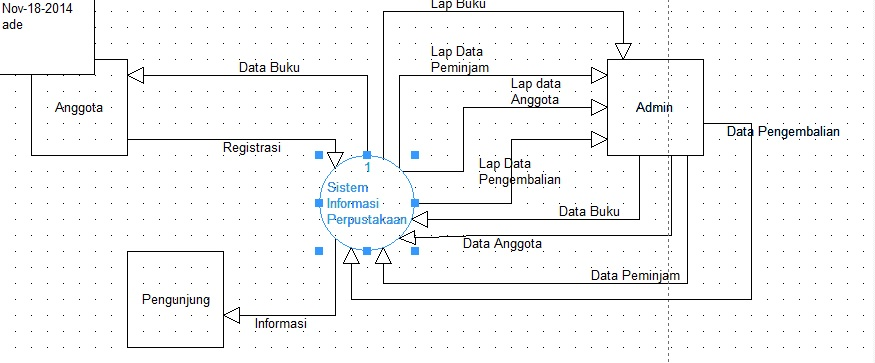
\includegraphics[width=1\textwidth]{gambar/DK}
    \caption{Diagram Konteks.}
    \label{DK}
\end{figure}
\newpage

\subsection{DFD level 1}
\begin{figure}[ht!]
  \centering
    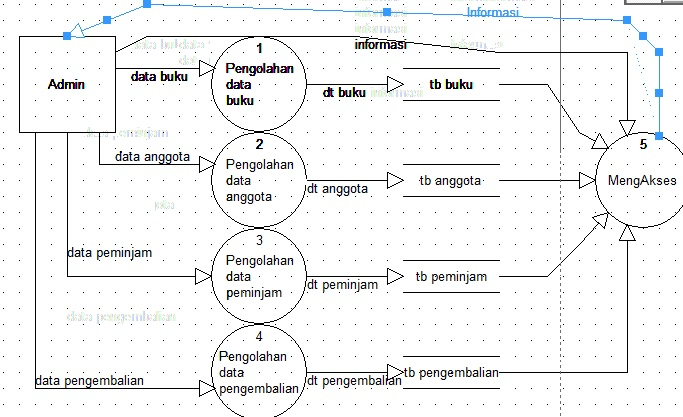
\includegraphics[width=1\textwidth]{gambar/lvl1}
    \caption{Dfd Level 1 Admin.}
    \label{lvl1}
\end{figure}
\newpage
\subsection{Flowchart Sistem}
\begin{figure}[ht!]
\centering
	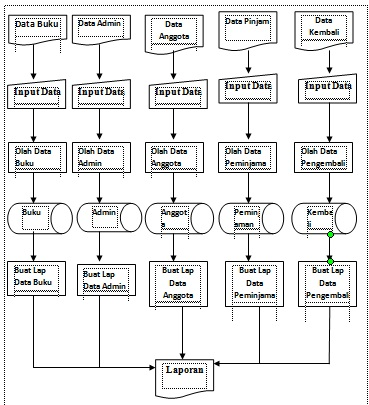
\includegraphics[width=1\textwidth]{gambar/Flowchart}
	\caption{Flowchart Sistem Informasi Perpustakaan.}
	\label{Flowchart}
\end{figure}
\newpage

\section{Jadwal Kegiatan}
Penelitian direncanakan akan dilaksanakan selama 6 bulan . Rincian rencana jadwal penelitian dicantumkan dalam tabel berikut.

\begin{center}
Tabel 3.1. Jadwal Penelitian.
\end{center}
\vspace{-0.5cm}
\begin{figure}[ht!]
  \centering
    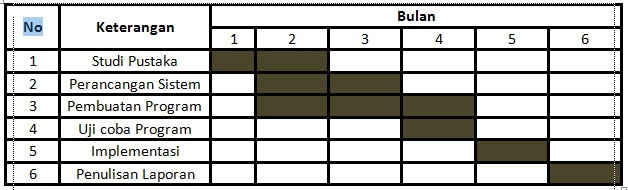
\includegraphics[width=1\textwidth]{gambar/JK}
\end{figure}

%-----------------------------------------------------------------
%Disini akhir masukan Bab
%-----------------------------------------------------------------

%-----------------------------------------------------------------
%Disini awal masukan untuk Daftar Pustaka
%-----------------------------------------------------------------
%%\nocite{Abel2010,Guerbas201350}
%%\bibliography{research-plan}
%%\bibliographystyle{plainnat}
\begin{thebibliography}{9}
\bibitem[satu(2013)]{satu01}
Kadir. Abdul. 2003. Pengenalan Sistem Informasi. Yogyakarta: Andi

\bibitem[dua(2013)]{dua02}
Nugroho. Bunafit. 2003. Database Relasional dengan MySql. Yogyakarta: Andi 

\bibitem[tiga(2013)]{tiga03}
P. Eko. 2008. Pemrograman Web PHP dan MySQL Untuk Sistem Informasi Perpustakaan. Yogyakarta : Graha Ilmu. 

\bibitem[empat(2013)]{empat04}
R.W, Renati. 2008. PHP dan MySQL Untuk Pemula. Yogyakarta : C.V Andi Offset. 
Sutarman. 2007. Membangun Aplikasi Web Dengan php dan MySQL. Yogyakarta :Graha Ilmu



\end{thebibliography}
\addcontentsline{toc}{chapter}{DAFTAR PUSTAKA}
%-----------------------------------------------------------------
%Disini akhir masukan Daftar Pustaka
%-----------------------------------------------------------------

\end{document}